Beide regionalen Klimamodelle wurden mit denselben Daten betrieben: Den Re-Analysedaten und den Simulationsdaten des GCM MPI-ESM-LR 
\section{MPI-ESM-LR} \label{sec:MPI}
Das globale Klimamodell des Max-Planck-Instituts MPI-ESM verbindet Atmosphäre, Ozean und Landoberfläche durch den Austausch von Energie, Momentum, Wasser und $CO_{2}$. Das Modell besteht aus einzelnen Komponenten: ECHAM6 für die Atmosphäre, MPIOM für den Ozean, JSBCACH für die Biosphäre der Landoberfläche und HAMOCC für die Biogeochemie des Ozeans. Für die Verbindung der gekoppelten Komponente HAMOCC und MPIOM zu den restlichen Komponenten über Energie, Momentum, Wasser und $CO_2$ wurde eine eigene Komponente OASIS3 eingeführt. Eine exemplarische Abbildung vom Aufbaus des Modells ist in der Abbildung \ref{fig:mpi-esm} zu sehen. Wegen der derzeitig beschränkten Rechenkapazitäten können komplexe GCMs nur mit einer relativ groben Auflösung von ca 120 -200 km berechnet werden. Für die Vorhersage von Auswirkungen der Klimaänderung benötigt es aber detailliert aufgelöste regionale Komponenten des Klimas. Es gibt mehrere Methoden für das Erhalten der regionalen Daten, wie z.B. RCMs, hoch auflösende GCMs, oder statistische Methoden.
\begin{figure}[h]
	\centering
	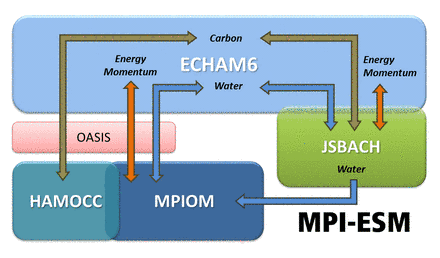
\includegraphics[width=0.7\textwidth]{mpi.png}
	\caption{Aufbau des MPI-ESM, von \cite{mpi-esm-lr}}
	\label{fig:mpi-esm}
\end{figure}
\section{Reanalysedaten}
Reanalysedaten entsprechen dem Abbild des globalen Klimas der Gegenwart oder der nahen Vergangenheit. Diese werden über globale Analysemodelle entwickelt, welche mit einem Zustand der Beobachtungsdaten starten und im Zuge der Simulation stets mit zusätzlichen Beobachtungsdaten gefüttert werden. Ziel dieser Modelle ist es, den physikalischen Annahmen treuen und den Beobachtungsdaten nahen Verlauf zu simulieren, um unter anderem die Güte der physikalischen Annahmen zu evaluieren.
\section{Downscaling-Methoden}
Downscaling hat den Zweck, die Auswirkungen der Daten aus einem globalen Klimamodell, mit einer Auflösung von ca. 120-200km auf regionaler Ebene zu berechnen. Dabei kann entweder eine empirisch statistische Herangehensweise verfolgt werden oder eine dynamisch Modellierte. Durch die empirisch statistischen Methode werden die Beziehungen zwischen der globalen Atmosphären-Konstellation und den regionalen Klimaverhältnissen statistisch quantifiziert. Die größte Herausforderung ist hierbei, geeignete Prädiktoren für den Zusammenhang zu finden. Da es sich bei beiden evaluierten Methoden nicht um Statistische sondern Dynamische handelt, wird nicht näher darauf eingegangen, eine genauere Beschreibung dieser Art von Methode findet man in \cite{RCM}, Kapitel 3. Die dynamische Methode hingegen ist eine
physikalisch basierte, räumliche Interpolation von GCM-Daten. Wie in Kapitel \ref{sec:MPI} erwähnt, gibt es mehrere Downscaling-Methoden:
\begin{enumerate}[label=(\alph*)]
	\item Vereinfachung eines globalen Klimamodells bzw. entkoppeln von sich relativ langsam anpassenden Komponenten z.B. der Ozean-Komponente, die dadurch gewonnene Rechenleistung kann in der höheren Auflösung angewendet werden.
	\item Globale Modelle durch eine variierende räumlichen Auflösung zu vereinfachen. Somit können einige regionale Gebiete höher aufgelöst modelliert werden.
	\item RCM: Die am häufigsten verwendete und in dieser Arbeit auch evaluierte Methode ist, das Einbetten eines räumlich begrenzten Modells in ein globales Modell. Die für das regionale Klimamodell benötigten zeitlich variablen Größen werden dem GCM entnommen und dem Gleichungssystem des RCMs als Randbedingungen zugeführt, somit verfügt das regionale Modelle stets über das aktuelle Abbild der Atmosphäre. Diese Größen müssen nicht zwangsläufig in nur eine Richtung fließen, es kann auch Informationen aus dem RCM zurück in das GCM fließen. Manche hybride RCMs können auch beides, ein und zweifache Flussrichtung der Informationen: von einem in sich selbst gebetteten RCM, fließt Information zum übergeordneten RCM, welches aber abgekapselt in einem GCM gebettet liegt. So kann die Auflösung sukzessive erhöht werden. 
\end{enumerate}
\subsection{Regionale Klimamodelle}
Der zentrale Baustein eines regionalen Klimamodells ist die atmosphärische Komponente, die Austauschvorgänge der Oberfläche werden durch ein interaktiv angekoppeltes Boden-Schnee-Vegetationsmodell erfasst (aus \cite{RCM} Kapitel 4.2f). Für die restliche Bausteine (siehe Abb. \ref{fig:mpi-esm}) werden im einfachsten Fall die vom GCM berechneten Simulationsdaten herangezogen, oder es werden Modelle entwickelt, welche z.B. die regionalen See- und Meeresprozesse nachbilden.\\
Die horizontal Auflösung des Gitters solcher Modelle liegt meist deutlich unter 50km bis zu unter einem km. Aus numerischen Gründen können nur Strukturen (z.B. Gewitterzellen) der vierfachen Gitterweite adäquat berechnet werden. Die vertikale Auflösung beträgt im Normalfall 30-60 Schichten, deren Höhe variiert. Bodennahe Schichten fallen meist dünner als Höhergelegene aus.\\
Im wesentlichen beruhen regionale sowie globale Modelle auf denselben physikalischen Prinzipien: Erhalt der Energie, Masse und des Impulses. Die Gleichungen der Komponenten unterscheiden sich jedoch aufgrund ihrer Formulierungen und besonders in deren Vereinfachungen. Die 
\subsection{CCLM4-8-17}


\subsection{CCLM5-0-9}